%%
%% ****** ljmsamp.tex 13.06.2018 ******
%%
\documentclass[
11pt,%
tightenlines,%
twoside,%
onecolumn,%
nofloats,%
nobibnotes,%
nofootinbib,%
superscriptaddress,%
noshowpacs,%
centertags]%
{revtex4}
\usepackage{ljm}
\graphicspath{{./images/}}
\begin{document}

%\titlerunning{?$\alpha$-спирали?} % for running heads
%\authorrunning{Орлов, Победин} % for running heads
%\authorrunning{First-Author, Second-Author} % for running heads

\title{?Что-то про $\alpha$-спирали?}
% Splitting into lines is performed by the command \\
% The title is written in accordance with the rules of capitalization.

\author{\firstname{Я.~?.}~\surname{Орлов}}
\affiliation{Физтех-школа физики и исследований им. Ландау. \\ Московский физико-технический институт (национальный исследовательский университет)}

\author{\firstname{Н.~К.}~\surname{Победин}}
\affiliation{Физтех-школа физики и исследований им. Ландау. \\ Московский физико-технический институт (национальный исследовательский университет)}
%\noaffiliation % If the author does not specify a place of work.

%\firstcollaboration{(Submitted by A.~A.~Editor-name)} % Add if you know submitter.
%\lastcollaboration{ }

\received{: \today} % The date of receipt to the editor, i.e. December 06, 2017


% \begin{abstract} % You shouldn't use formulas and citations in the abstract.
% In this example, the article contains some required author
% information and examples of how to gain an article in the REV\TeX~4
% for \ljm. You shouldn't use formulas and citations in the abstract.
% \end{abstract}

%\subclass{12345, 54321} % Enter 2010 Mathematics Subject Classification.

\keywords{$\alpha$-спираль, ?} % Include keywords separeted by comma.

\maketitle

% Text of article starts here.
\section{Введение}
?какой-то текст про цели задачи туда сюда?
\section{Теоретические сведения}
\subsection{Понятие о структуре белков}
Белки — это и молекулярные машины, и строительные блоки, и оружие живой клетки. Важнейшая и почти монопольная функция белков - ферментативный катализ химических превращений в клетке и вокруг нее. 

\begin{wrapfigure}[17]{r}{6cm}
	\centering
	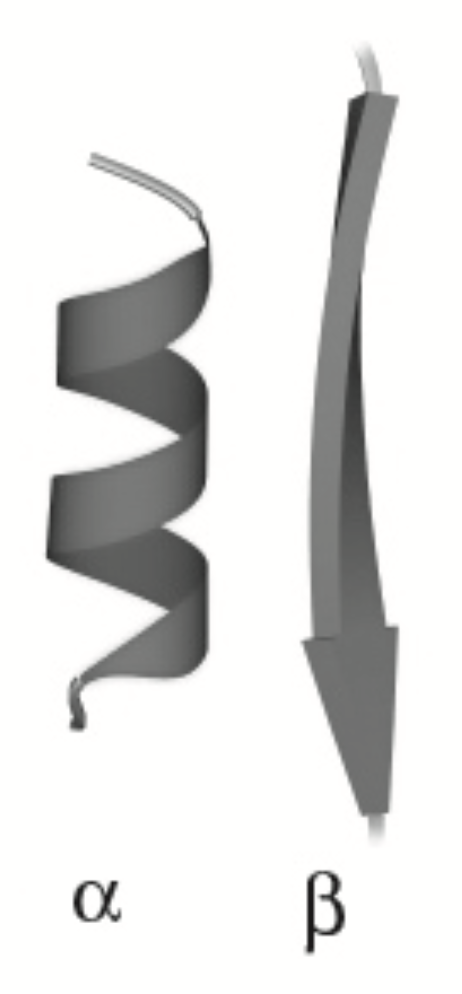
\includegraphics[scale=0.3]{alpha}
	\caption{$\alpha$-спираль и $\beta$-структура}
\end{wrapfigure}
При всем разнообразии, работа белков всегда базируется на высоко специфическом — как у ключа с замком (точнее: как у гибкого ключа с гибким замком) - взаимодействии белка с обрабатываемой им молекулой. Для этого взаимодействия необходима достаточно «твердая» (во всяком случае, у «работающего белка) пространственная структура. Поэтому биологическая функция белков (как и других важнейших для жизни макромолекул — ДНК и РНК) тесно связана с определенностью их трехмерных структур. Не только разрушение - даже небольшие изменения этих структур часто ведут к утере или резкому изменению активности белков.
Знание молекулярной трехмерной структуры белка необходимо для понимания функционирования белковой молекулы. 

Нековалентные взаимодействия, поддерживающие пространственное строение белка, значительно слабее химических связей, фиксирующих последовательность мономеров — аминокислот в белковой цепи. Эта
последовательность — она называется «первичной структурой белка» (рис. 1) — создается в ходе матричного биохимического синтеза согласно «инструкции», записанной в гене.

Архитектуры белков сложны и разнообразны — в противоположность универсальности двойной спирали ДНК. Однако и в белках прослеживается набор «стандартных» структур.
В своей работе мы будем исследовать $\alpha$-спирали, которые часто изображаются спиральными лентами или цилиндрами (рис. 1)


\subsection{Карты Рамачандрана}

Аминокислоты связанны между собой пептидными связями C' и N атомов
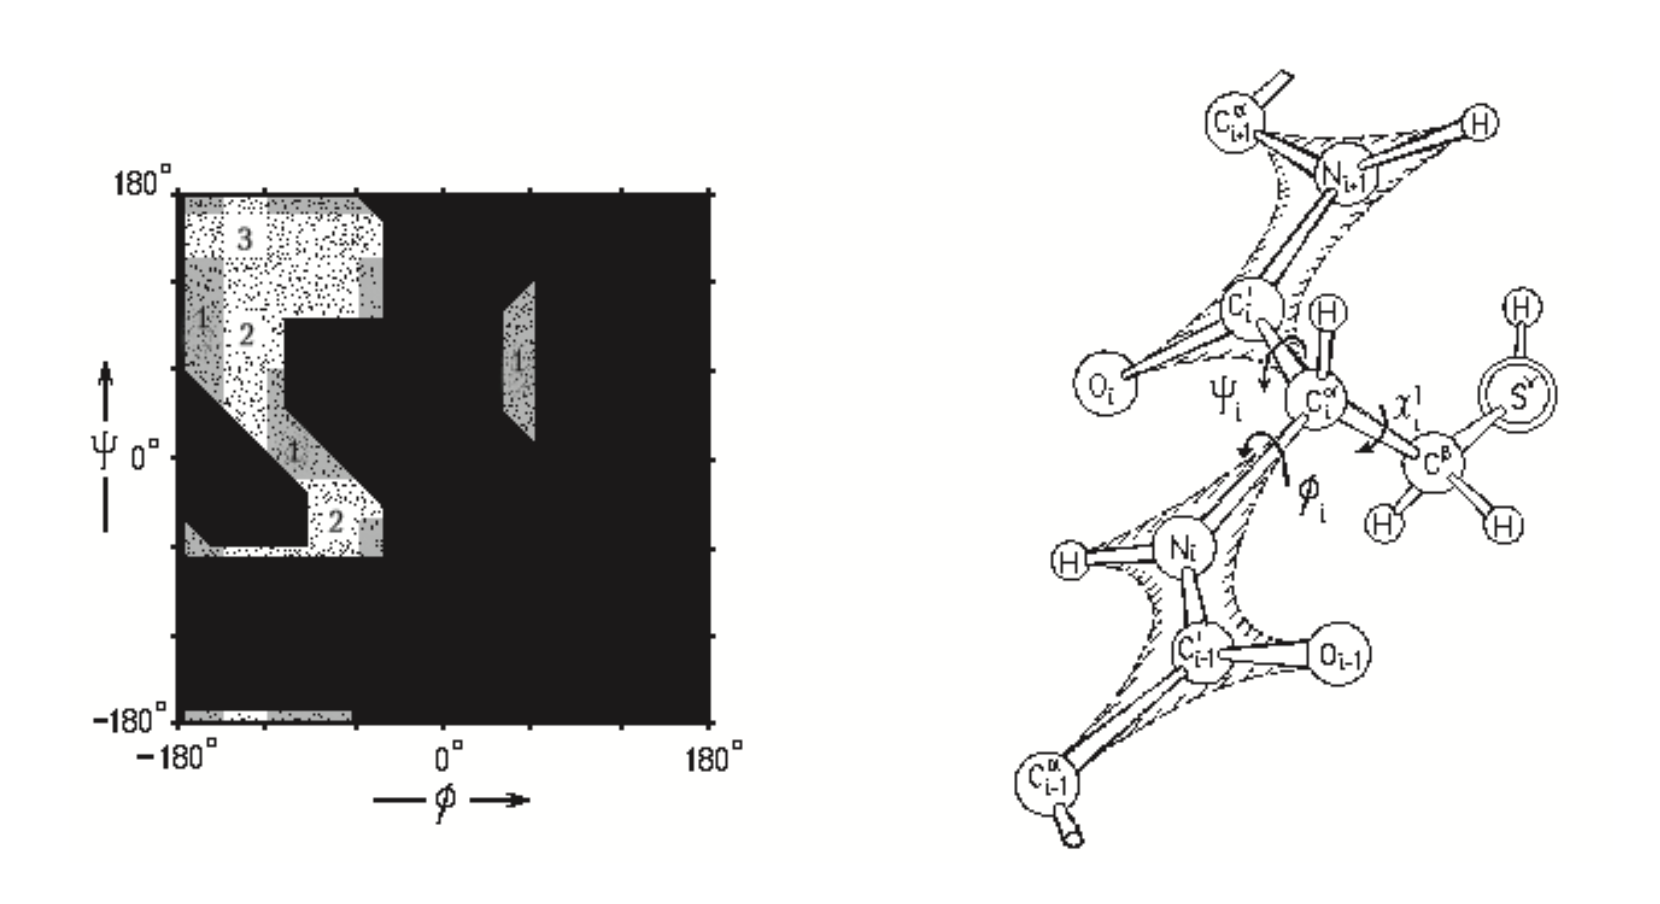
\includegraphics[width=\textwidth]{map}
На рисунке 2 справа изображен полипептид: главная цепь и боковая группа (Ser) на ней. Пептидные группы заштрихованы. Показаны углы внутреннего вращения в главной $(\phi, \psi, \omega)$ и боковой ( $\chi^1$ ) цепях. Индексы $i-1, i, i+1$ показывают последовательность аминокислотных остатков в цепи. Стрелки указывают направление вращения ближней к нам части цепи относительно более отдаленной ее части, ведущее к росту угла поворота. 

Слева изображена его карта Рамачандрана - изображенные в координатах ($\phi$, $\psi$) запрещенные и разрешенные конформации (то есть положения при повороте на на углы $\phi$ и $\psi$) остатка. 


Рис. 3-5. Карта запрещенных ($\blacksquare$) и разрешенных ( $\square$, I - точки на белом фоне, II - точки на сером фоне) конформаций крупных остатков при вращении по углам $\phi, \psi$ в белковой цепи. В области $\square$ разрешены все три ротамера $C^{\gamma}$ атома по $\chi^{1}$, в области II - 2 ротамера, в области I - 1 ротамер.
\newpage
\subsection{Свойства аминокислотных остатков}
Список 20 «стандартных», т. е. кодируемых ДНК-аминокислотных остатков дан в таблице ниже, там же дан их молекулярный вес и встречаемость в белках. Структуры этих аминокислотных остатков представлены на рис. 2.
\begin{table}[!ht]
	\begin{tabular}{|c|c|c|c|c|c|c|c|c|c|c|c|c|c|}
		\hline \multirow{3}{*}{\begin{tabular}{l} 
				A.к. \\
				ост. \\
		\end{tabular}} & \multicolumn{2}{c|}{Наличие} & Число & Диполь/заряд & $\mathrm{pK}$ & \multicolumn{8}{c|}{ Яркая тенденция быть: } \\
		& $\mathrm{NH}$ & $\mathrm{C}^\beta$ & $\gamma$ & & & до- & \multicolumn{3}{c|}{В спирали}& зa- & в & в & в \\
		& & & б.гр. & & & $\alpha_{\mathrm{N}}$ & $\alpha_{\mathrm{N}}$ & $\alpha$ & $\alpha_{\mathrm{C}}$ & $\alpha_{\mathrm{C}}$ & $\beta$ & петлях & ядре \\
		\hline Gly & $+$ & $-$ & & & & & & \boldmath$-$ & & & $-$ & \boldmath$+$& \\
		\hline Ala & $+$ & $+$ & & & & & & \boldmath$+$ & & & & $-$ & \\
		\hline Pro & $-$ &$+$ & 1 & & & & \boldmath$+$ & \boldmath$-$ & \boldmath$-$ & \boldmath$-$ & \boldmath$-$ & \boldmath$+$ & \\
		\hline Glu & $+$ & $+$ & 1 & $\mathrm{COOH} \Rightarrow \mathbf{C O}_2^{-}$ & 4,3 & \boldmath$+$ & \boldmath$+$ & & \boldmath$-$ & \boldmath$-$ & $-$ & & $-$ \\
		\hline Asp & $+$ & $+$ & 1 & $\mathrm{COOH} \Rightarrow \mathbf{C O}_2^{-}$ & 3,9 & \boldmath$+$ & \boldmath$+$ & $-$ & \boldmath$-$ & \boldmath$-$ & \boldmath$-$ & $+$ & \boldmath$-$ \\
		\hline Gln &$+$ & $+$ & 1 & $\mathrm{OCNH}_2$ & & & & & & & & & $-$ \\
		\hline Asn & $+$ & $+$ & 1 & $\mathrm{OCNH}_2^2$ & & $+$ & & \boldmath$-$ & & $+$ & \boldmath$-$ & \boldmath$+$ & $-$ \\
		\hline Ser & $+ $& $+$ & 1 & $\mathrm{OH}$ & & $+$ & & & & & & $+$ & $-$ \\
		\hline His & $+$ & $+$ & 1 & $\mathbf{N H} ;$ и $\mathbf{N} \Rightarrow \mathbf{N H}^{+}$ & 6,5 & & $-$ & & $+$ & $+$ & & & \\
		\hline Lys & $+$ & $+$ & 1 & $\mathrm{NH}_2 \Rightarrow \mathbf{N H}_3^{+}$ & 10,5 & \boldmath$-$ & \boldmath$-$ & & \boldmath$+$ & \boldmath$+$ & $-$ & & $-$ \\
		\hline Arg & $+$ & $+$ & 1 & $\mathbf{H N C}\left(\mathbf{N H}_2\right)_2^3+$ & 12,5 & \boldmath$-$ & \boldmath$-$ & & \boldmath$+$ & \boldmath$+$ & \boldmath$-$ & $+$ & \boldmath$-$ \\
		\hline Thr & $+$ & $+$ & 2 & $\mathrm{OH}$ & & $+$ & & & & & \boldmath$+$ & & \\
		\hline Ile & $+$ & $+$ & 2 & & & & & & & & \boldmath$+$ & $-$ & \boldmath$+$ \\
		\hline Val & $+$ & $+$ & 2 & & & & & & & & \boldmath$+$ & $-$ & \boldmath$+$ \\
		\hline Leu & $+$ & $+$ & 1 & & & & & \boldmath$+$ & & & $+$ & \boldmath$-$ & \boldmath$+$ \\
		\hline Met & $+$ & $+$ & 1 & & & & & \boldmath$+$ & & & \boldmath$+$ & \boldmath$-$ & \boldmath$+$ \\
		\hline Phe & $+$ & $+$ & 1 & & & & & & & & $+$ & $-$ & \boldmath$+$ \\
		\hline Tyr &$+$ & $+$ & 1 & $\mathbf{O H} \Rightarrow \mathrm{O}^{-}$ & 10,1 & & &$-$ & & & $+$ & & $+$ \\
		\hline Cys & $+$ & $+$ & 1 & $\mathbf{S H} \Rightarrow \mathbf{S}^{-}$ & 9,2 & & & $-$ & & & $+$ & & \boldmath$+$ \\
		\hline Trp & $+$ & $+$ & 1 & $\mathrm{NH}$ & & & & & & & $+$ & & $+$ \\
		\hline
	\end{tabular}
\end{table}
\begin{figure}[!ht]
	\centering
	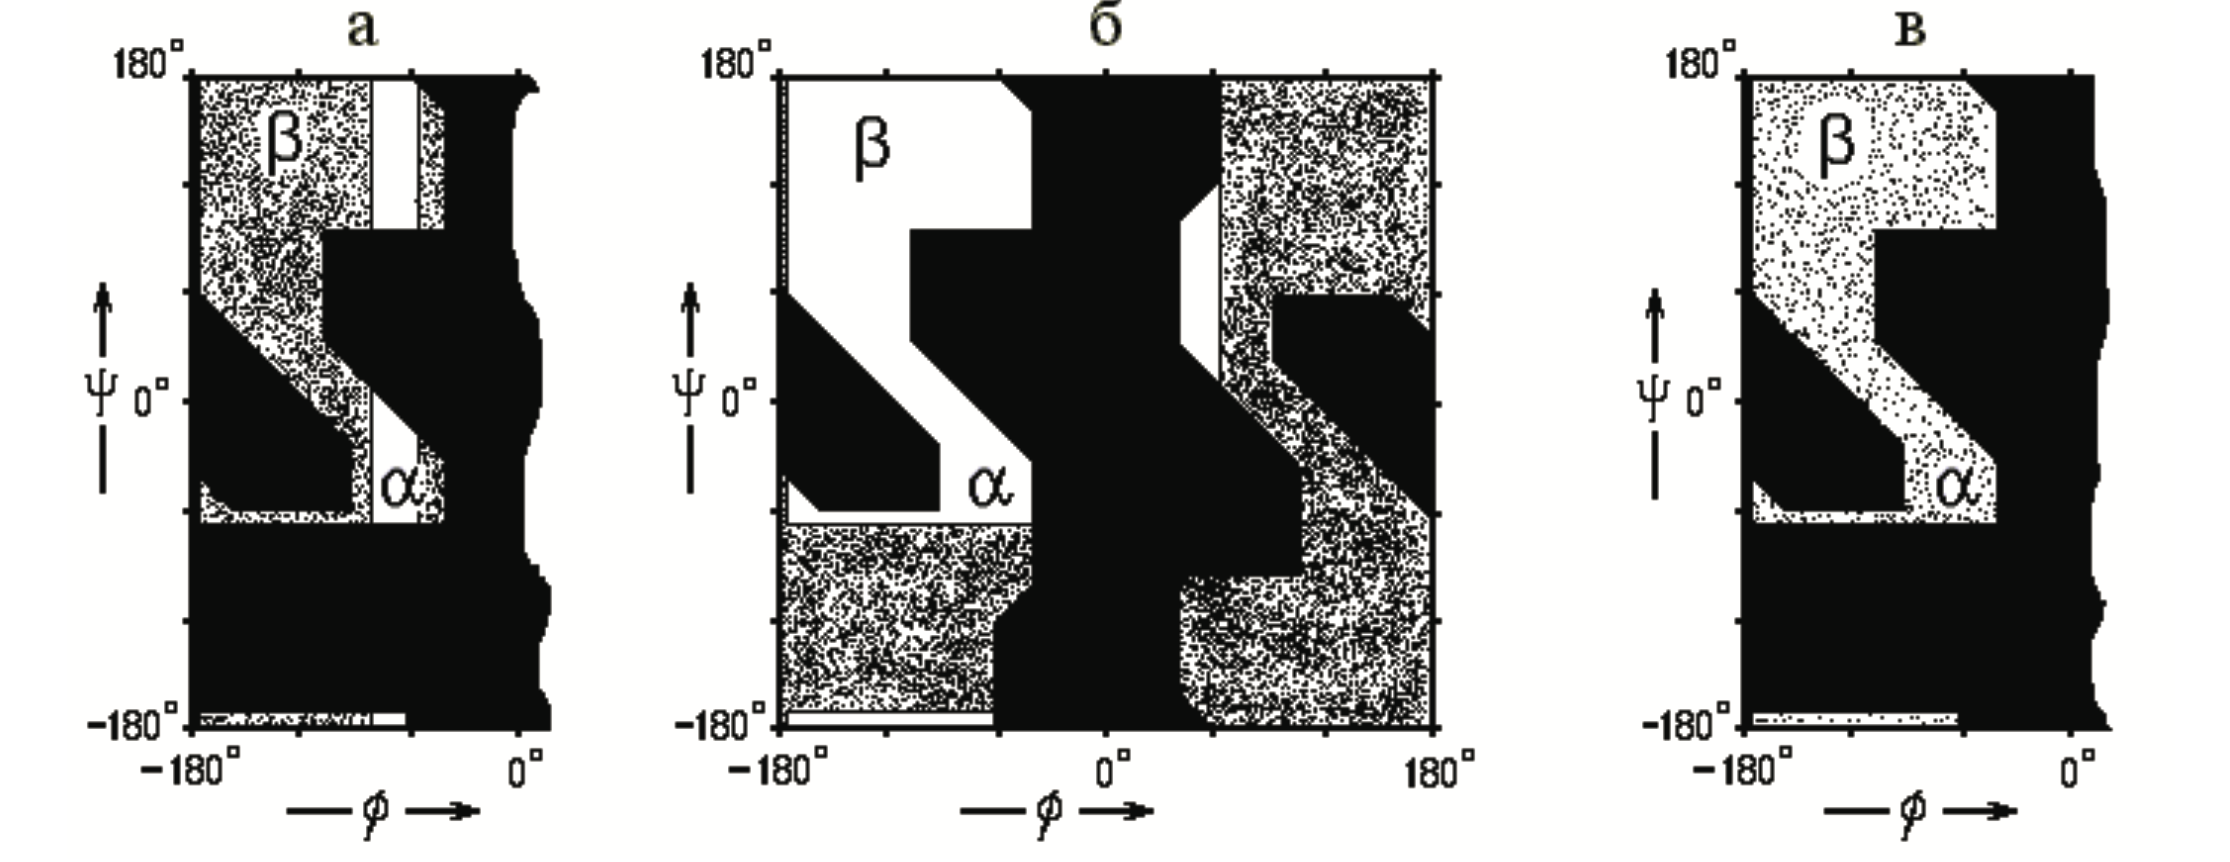
\includegraphics[width=\textwidth]{zone}
	\caption{Запрещенные и разрешенные конформации различных аминокислотных остатков и - на их фоне - конформации $\alpha$ - и $\beta$-структуры. (а) Разрешенные для пролина конформации ( $\square$ ) на фоне конформаций, разрешенных для аланина (I - точки на белом фоне); $\blacksquare$- конформации, запрещенные для них обоих. (б) Разрешенные конформации аланина ( $\square$ ) на фоне конформаций I, разрешенных лишь для глицина; $\blacksquare$ — области, запрещенные для всех остатков. (в) Карта запрещенных ($\blacksquare$) и разрешенных ($\square$, I) конформации боковой группы по углу $\chi^1$, в области I часть углов $\chi^1$ запрещена}
\end{figure}

Попробуем понять основные закономерности этой таблицы, исходя из того, что мы уже изучили. При этом мы будем использовать следующую логику: так как белок в целом стабилен, он должен в основном состоять из стабильных элементов, т.е. именно они должны наблюдаться в его структуре чаще всего, а нестабильные должны наблюдаться редко.

Почему пролин не любит вторичной структуры? Потому, что у него нет зывать водородные связи, а именно на них и держится вторичная структуpa. Почему он, тем не менее, любит N-конец спирали? Потому, что здесь, в водородные связи, и здесь пролину нечего терять... С другой стороны, угол $\varphi$ в пролине фиксирован его кольцом примерно при $-60^{\circ}$, т. е. его конформация уже почти «готова» для $\alpha$-спирали (рис. 10-2a).


Почему глицин не любит вторичной структуры и предпочитает нерегулярные участки («клубок»)? Потому, что для него допустима очень широкая область углов ( $\varphi \psi$ ) на карте Рамачандрана (рис. 10-2б), ему легко принимать самые разнообразные конформации, лежащие вне вторичной структуры.

\begin{wrapfigure}[18]{r}{7cm}
	\centering
	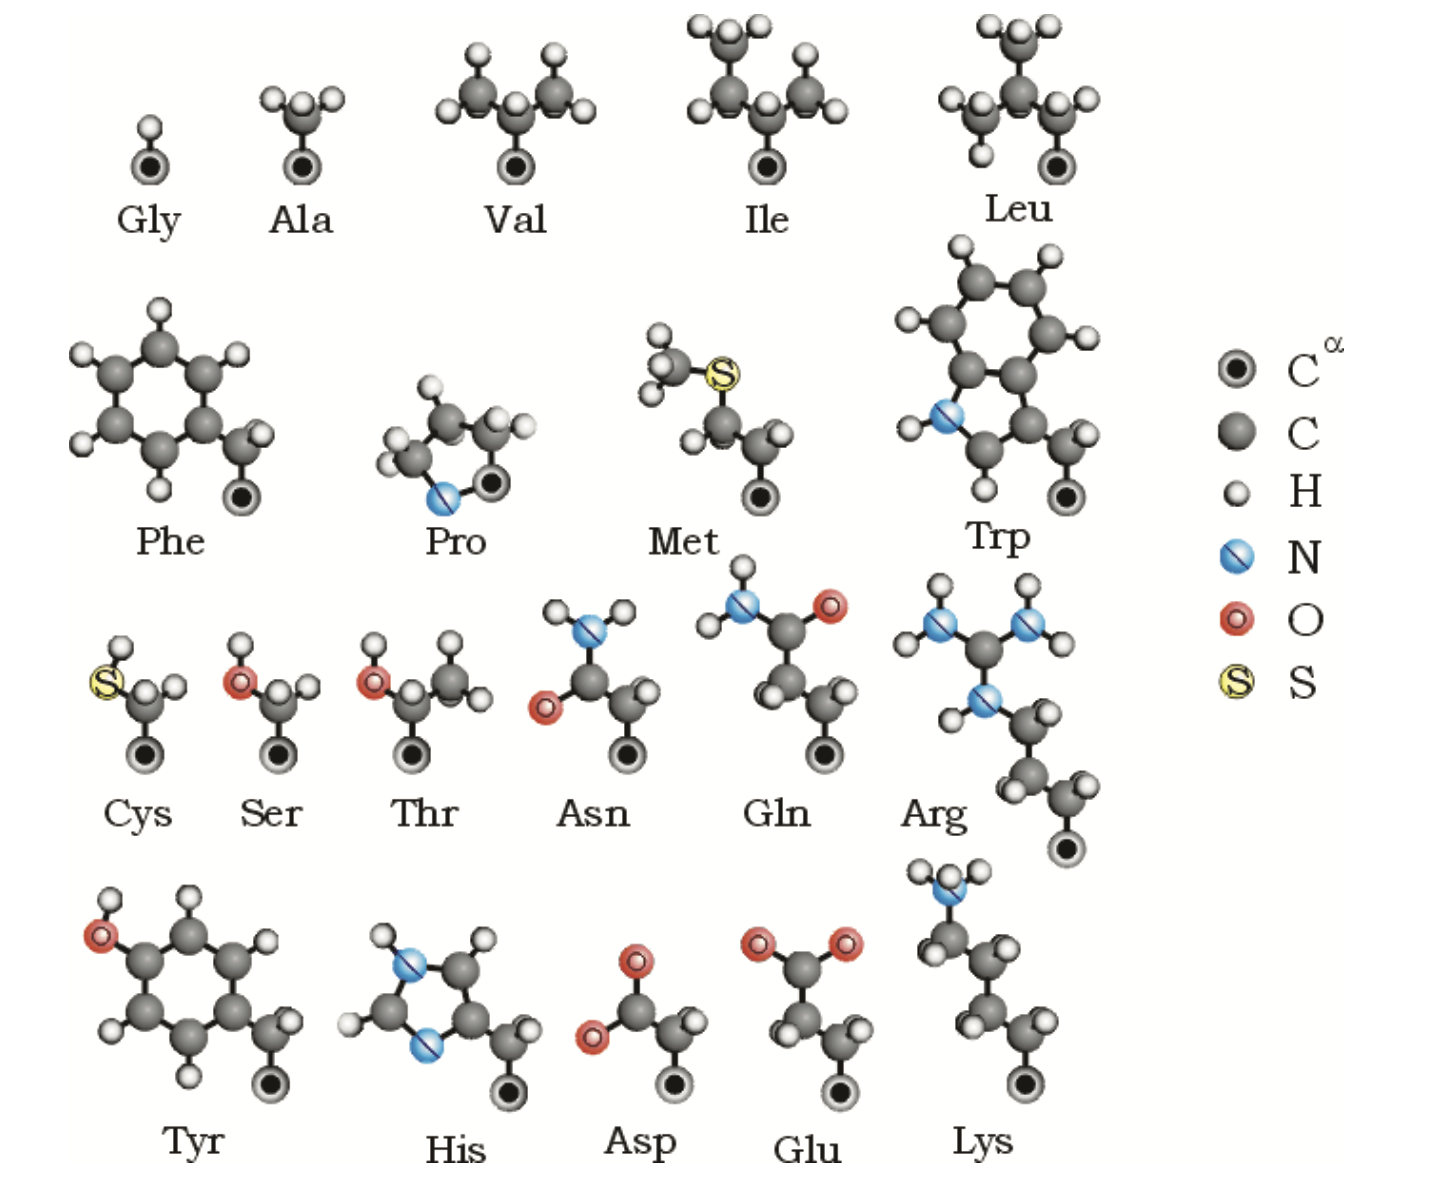
\includegraphics[scale=0.3]{amin}
	\caption{}
\end{wrapfigure}
Наоборот, аланин - с более узкой, но включающей и $\alpha-$, и $\beta$-конформацию разрешенной областью на карте Рамачандрана (рис. 10-2б) - предпочитает нерегулярным конформациям $\alpha$-спираль (и отчасти $\beta$-структуру).

Остальные гидрофобные остатки (т.е. остатки без зарядов и диполей в боковой цепи) предпочитают, как правило, $\beta$-структуру. Почему? Потому, что их крупные $\gamma$-атомы могут там располагаться более свободно (рис. 10-2в). Особенно это важно для боковых групп с двумя крупными $\gamma$-атомами.

А вот аминокислоты с полярными группами в боковых цепях предпочитают поверхностные нерегулярные участки («клубок»), где эти полярные группы могут завязать водородные связи как с полипептидной цепью, так и с водой. Особенно заметна эта тенденция для наиболее полярных, заряженных при «нормальном» рН7 остатков, и для самых коротких (см. рис. 10-1) полярных боковых цепей, с наиболее приближенными к главной цепи полярными группами. Кстати, по той же причине, поскольку у них там есть возможность завязать дополнительную водородную связь, короткие полярные боковые группы любят места у обоих концов спирали.

Некое исключение среди аминокислот с диполями в боковой цепи составляют триптофан и тирозин, имеющие маленький диполь на фоне большой гидрофобной части, и цистеин, у которого (т.е. у SH-группы которого) водородные связи совсем слабые. Они ведут себя, в общем, так же, как гидрофобные остатки.

Мы видим также, что отрицательно заряженные боковые группы предпочитают $\mathrm{N}$-конец спирали (точнее: $\mathrm{N}$-концевой виток и один-два остатка перед ним) и не любят С-концевой виток (и пару остатков за ним), а положительно заряженные - предпочитают С-конец спирали и не любят ее $\mathrm{N}-$-онец. Почему? Потому, что на N-конце из спирали торчат NH-группы и на нем образуется заметный положительный заряд, и «минусы» боковых цепей притягиваются к нему, а «плюсы» отталкиваются от него. А С-конец спирали заряжен, наоборот, отрицательно, и там эффект противоположен: около С-конца любят собираться «плюсы» боковых цепей, а «минусы» его избегают.


Что касается расположения остатков внутри белка или на его поверхности, здесь общая тенденция заключается в том, что полярные (гидрофильные) боковые группы находятся снаружи, где они могут контактировать с полярной же водой («подобное растворяется в подобном»!). Отрываться от воды полярным группам плохо - теряются водородные связи. Особенно плохо отрываться заряженным группам: переход из среды с высокой диэлектрической проницаемостью (из воды) в среду с низкой (ядро белка) ведет к большому повышению свободной энергии. И действительно, ионизированных групп внутри белка практически нет (а почти все исключения связаны либо с координационными связями с ионом металла, либо с активными центрами, ради которых, собственно, белок и создан...).

Наоборот, большинство гидрофобных боковых групп находятся внутри белка - они-то и создают здесь гидрофобное ядро (опять: «подобное растворяется в подобном»!). Мы уже говорили, что гидрофобность группы тем больше, чем больше ее неполярная поверхность: именно ее нужно упрятать от воды. Для чисто неполярных групп гидрофобный эффект прямо пропорционален их поверхности, а для групп с полярными вкраплениями - их поверхности за вычетом поверхности этих вкраплений.

Слипание гидрофобных групп - главная движущая сила образования белковой глобулы. Главная, но не единственная - еще есть образование водородных связей во вторичной структуре (о чем мы уже говорили) и образование плотной, квазикристаллической упаковки внутри белка (о чем мы еще поговорим в свое время).

Для создания гидрофобного ядра белковой цепью она должна входить в него с уже насыщенными водородными связями - ведь иначе ее полярным пептидным группам от воды придется оторваться, а разрыв водородной связи дорог. Поэтому в гидрофобное ядро вовлекается цепь, уже образовавшая (или образующая при этом) вторичную структуру и тем самым насытившая водородные связи пептидных групп в главной цепи. Однако при этом в ядро должны увлекаться только гидрофобные остатки вторичной структуры, а входящие в нее полярные остатки должны остаться вне ядра, потому и на $\alpha$-спиралях, и на $\beta$-структурных участках выделяются гидрофобные и гидрофильные поверхности; для их создания необходимо определенное чередование соответствующих групп в белковой цепи.

Все закономерности, о которых мы сейчас говорили, используются как для конструирования искусственных белков, так и для предсказания - по аминокислотным последовательностям - вторичной структуры белков, а также для предсказаний тех участков их цепи, что глубоко погружены в белок, или, наоборот, тех участков, что лежат на поверхности белка.

\newpage
\subsection{Стабильность $\alpha$-спирали}
Первая водородная связь в $\alpha$-спирали $(\mathrm{CO})_0-(\mathrm{HN})_4$ фиксирует конформации трех остатков - $1,2,3$; следующая водородная связь $(\mathrm{CO})_1-(\mathrm{HN})_5$ дополнительно фиксирует конформацию только одного остатка - остатка 4 ; связь $(\mathrm{CO})_2-(\mathrm{HN})_6$ дополнительно фиксирует остаток 5 , и т. д.

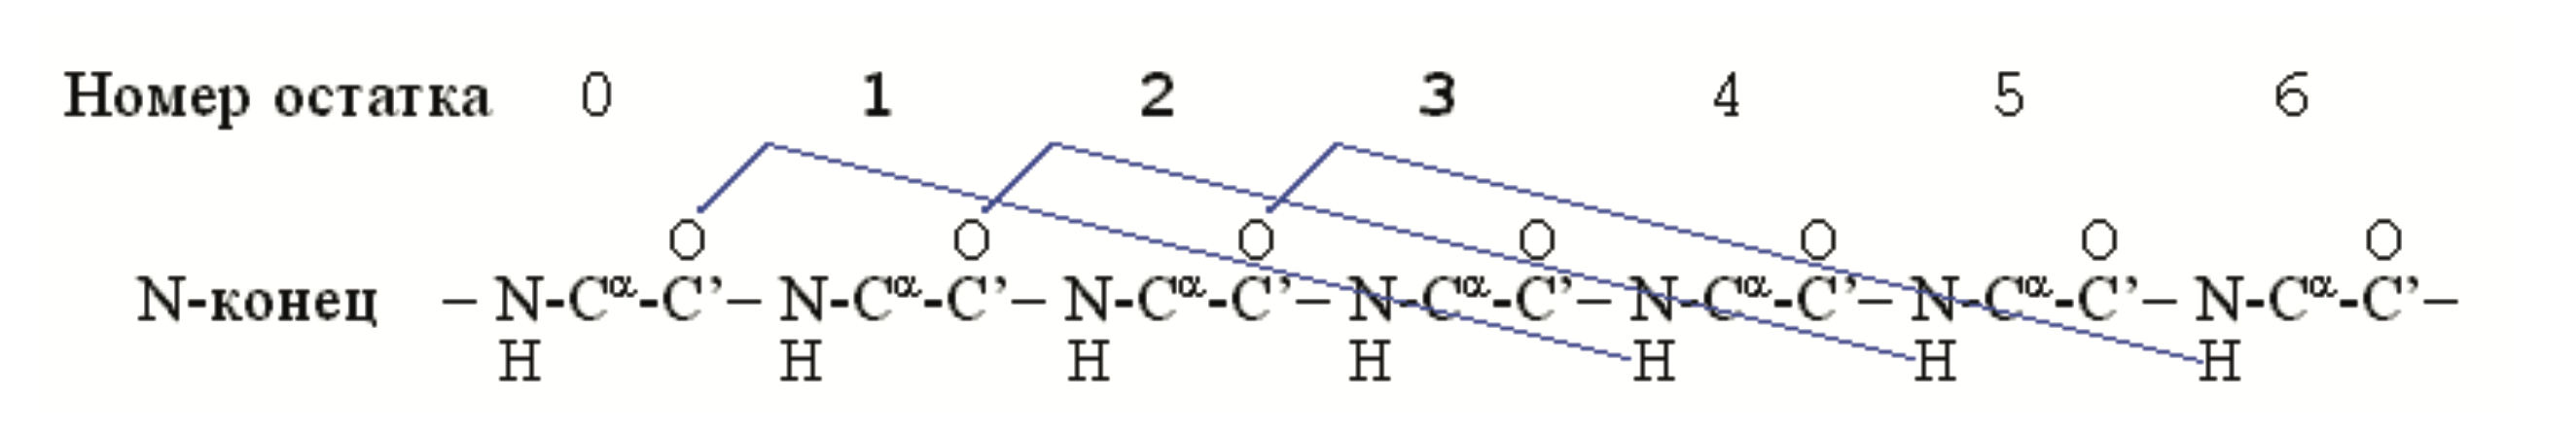
\includegraphics[width=\textwidth]{ostatok}

Значит, если в спирали фиксировано $n$ остатков, то их фиксирует $n-2$ водородные связи. Рассмотрим свободную энергию образования такой спирали из клубка в водном окружении («клубок» - это полимер без фиксированной структуры и без взаимодействия дальних по цепи звеньев). Эту свободную энергию можно записать как
\begin{equation}
	\Delta F_\alpha=F_\alpha-F_{\text {клуб. }}=(n-2) f_{\mathrm{H}}-\mathrm{n} T S_\alpha=-2 f_{\mathrm{H}}+n\left(f_{\mathrm{H}}-T S_\alpha\right) .
\end{equation}

Здесь $f_{\mathrm{H}}$ - свободная энергия образования водородной связи и сопутствующих ей взаимодействий в $\alpha$-спирали (вы помните, что $f_{\mathrm{H}}-$ не просто энергия, как было бы в вакууме: в нее входит и энергия, и энтропия перестроек водородных связей в водном окружении), а $S_\alpha$ - потеря энтропии при фиксации одного остатка в спирали.

Вы видите, что в $\Delta F_\alpha$ есть два члена. Один ( $-2 f_{\mathrm{H}}$ ) не зависит от длины спирали; величина
\begin{equation}
	f_{\text {init }}=-2 f_{\mathrm{H}}
\end{equation}

традиционно называется свободной энергией инициации спирали (на самом деле, $f_{\text {init }}$ - суммарная свободная энергия обеих границ спирали с клубком; она учитывает и инициацию, и терминацию спирали). Другой член, $n\left(f_{\mathrm{H}}-T S_\alpha\right)$, прямо пропорционален длине спирали; величина
\begin{equation}
	f_{\mathrm{el}}=\left(f_{\mathrm{H}}-T S_\alpha\right)
\end{equation}

называется свободной энергией элонгации спирали на один остаток. В общем виде
\begin{equation}
	\Delta F_\alpha=f_{\text {init }}+n f_{\text {el }} .
\end{equation}

При этом отношение вероятности чисто спирального состояния цепи из $n$ остатков к ее же чисто клубковому (и начисто лишенному спиральных примесей) состоянию, равно
\begin{equation}
	\exp \left(-\Delta F_\alpha / k T\right)=\exp \left(-f_{\text {init }} / k T\right)\left[\exp \left(-f_{\mathrm{el}} / k T\right)\right]^{\mathrm{n}}=\sigma s^{\mathrm{n}} .
\end{equation}

Здесь используются общепринятые обозначения:
\\- фактор элонгации спирали: $s=\exp \left(-f_{\mathrm{el}} / k T\right)$;
\\- фактор инициации спирали: $\sigma=\exp \left(-f_{\text {init }} / k T\right)$.

Ясно, что $\sigma<<1$, так как $\sigma=\exp \left(-f_{\text {init }} / k T\right)=\exp \left(+2 f_{\mathrm{H}} / k T\right)$; а свободная энергия водородной связи - большая отрицательная величина, порядка нескольких $k T$.

Величина $\exp \left(-\Delta F_\alpha / k T\right)=\sigma s^n$ — это просто константа равновесия $n$ звеньев.

Выясним вопрос о том, как образуется спираль при изменении условий среды (температуры, растворителя и т. д.) - фазовым переходом или постепенно?
Поначалу кажется, что такая отличная от клубка структура, как спираль, должна «вымораживаться» из него путем фазового перехода — как лед из воды...
Однако на этот счет есть теорема Ландау, которая гласит, что в системе, где обе фазы одномерны, — фазовый переход первого рода невозможен.

"Одномерность" означает, что свободная энергия (или по сути размер границы раздела) не зависит размера кусков фаз. Соответственно в трехмерной системе сосуществование двух разных фаз энергетически не выгодно, а в одномерной выгодно. Поэтому в одномерной системе фазы перемешиваются. 
\\ \\Найдем характерную длину $n_0$ спирального участка в середине перехода спираль-клубок

Рассмотрим цепь из $N$ звеньев при температуре «середины перехода», где спираль и клубок имеют равную свободную энергию, т. е. $f_{\mathrm{el}}=0$. При этом свободная энергия элонгации спирали (а равно и клубка) - ноль, ее инициации - $f_{\text {init }}$, а число возможных положений спирали в цепи из $N$ звеньев - порядка $N^2 / 2$ (она может начинаться и кончаться в любом месте при единственном условии, что ее длина - не менее трех остатков); и ни расположение спирали в цепи, ни ее длина (при $f_{\mathrm{el}}=0$ ) не влияют на ее свободную энергию. Для получения качественной оценки пренебрежем мелочами (цифрами) по сравнению с главным (буквами). Итак: размещений спирали - порядка $N^2$, т. е. их энтропия - $k \cdot 2 \ln (N)$, а полная свободная энергия внедрения куска новой фазы (спирали с флуктуирующими концами) в цепь длины $N$ - примерно $f_{\text {init }}-2 k T \ln (N)$. Если она, эта свободная энергия, больше нуля - новая фаза не внедрится; если она меньше нуля - новая фаза может внедриться, и даже неоднократно. Значит, смешение клубковой и спиральной фаз начинается в кусках длины $N \sim n_0$, а величина $n_0$ получается из уравнения $f_{\text {init }}-2 k T \ln \left(n_0\right)=0$. Итак: характерная длина кусков спирали и клубка в середине перехода
\begin{equation}
	n_0=\exp \left(+f_{\text {init }} / 2 k T\right)=\sigma^{-1 / 2}
\end{equation}

Наконец, зная $n_0$, можно вычислить $f_{\text {init }}$ и $\sigma$. Для большинства аминокислот $n_0 \approx 30, f_{\text {init }} \approx 4$ ккал/моль, и $\sigma \approx 0,001$.

Теперь мы можем найти свободную энергию образования водородной связи (вкупе со всеми сопутствующими образованию Н-связи в $\alpha$-спирали взаимодействиями): согласно (2), $f_{\mathrm{H}}=-f_{\text {init }} / 2 \approx-2$ ккал/моль. Можно найти и конформационную энтропию, теряемую при фиксации одного звена в $\alpha$-спирали: согласно формуле (3), при $f_{\mathrm{el}}=0, T S_\alpha=f_{\mathrm{H}} \approx-2$ ккал/моль.

Оба параметра стабильности спирали - и $f_{\text {el }}^\alpha$, и $f_{\text {init }}$ - зависят от температуры, но по-настоящему сильно влияет на стабильность спирали именно отклонение величины $f_{\text {el }}$ от 0 . Дело в том, что в спирали, состоящей из $\sim n_0$ звеньев, это отклонение умножается на большое число $n_0$ и уже в таком виде входит в свободную энергию спирали. Когда величина $f_{\text {el }} n_0 / k T$ составляет порядка +1 (более точная оценка: $f_{\mathrm{el}} n_0 / k T=+2$ ), спиральность практически исчезает, а когда $f_{\mathrm{el}} n_0 / k T=-2-$ практически исчезает клубок. 

Стабильность $\alpha$-спирали обычно падает с ростом температуры и с добавлением полярных денатурантов и растет с добавлением слабополярных растворителей.

Для измерения влияния отдельных аминокислотных остатков на стабильность спиралей сейчас чаще всего используются короткие (длиной $\sim n_0$ или менее) полипептиды. В них может образоваться только одна спираль, и оценить влияние каждой аминокислотной замены на спиральность здесь наиболее просто. 

%
% The Bibliography
%

\begin{thebibliography}{99}
\bibitem{texbook}
\refitem{book}
Финкельштейн А. В., Птицын О. Б. \emph{Физика белка:} (Addison-Wesley, London, 1984).




\end{thebibliography}
\end{document}
